\documentclass[a4paper,11pt]{article}
\input{/home/tof/Documents/Cozy/latex-include/preambule_lua.tex}
\newcommand{\showprof}{show them}  % comment this line if you don't want to see todo environment
\fancyhead[L]{Ma première page web}
\newdate{madate}{10}{09}{2020}
\fancyhead[R]{Seconde - SNT} %\today
\fancyfoot[L]{~\\Christophe Viroulaud}
\fancyfoot[C]{\textbf{Page \thepage}}
\fancyfoot[R]{\includegraphics[width=2cm,align=t]{/home/tof/Documents/Cozy/latex-include/cc.png}}

\begin{document}
\begin{Form}
\section{Problématique}
Afin de préparer au mieux leur orientation, les élèves de seconde doivent réfléchir très tôt aux choix qu'ils devront effectuer (spécialités en classe de première, études post-baccalauréat, métier...). Le conseiller d'orientation du lycée leur demande de créer une page web présentant leur projet de parcours, à la manière d'un CV en ligne.
\section{Internet ou web?}
Comme nous l'avons vu précédemment \emph{internet} est la structure physique qui permet de relier tous les ordinateurs entre eux.
\begin{commentprof}
Contexte historique\\
Tim Berners-Lee: travaille au CERN (Conseil Européen pour la Recherche Nucléaire); rassemble les technologies (TCP/IP, réseau ARPANET, hypertexte) pour en faire un ensemble: WWW. a pour ambition initiale le partage sur un seul réseau de toutes les informations afin de faciliter la communication et les travaux des physiciens du CERN.\\
Uniform Ressource Identifier, HyperText Transfer Protocol, HyperText Markup Language
\end{commentprof}

Ce réseau permet de transformer tout type d'information:
\begin{itemize}
\item des mails,
\item des fichiers,
\item des vidéos,
\item des pages web.
\end{itemize}
Une \emph{page web} est un fichier écrit dans le langage \emph{html} (le plus souvent). Le \emph{navigateur} lit les instructions de la page pour afficher un rendu à l'écran.
Le \emph{World Wide Web} (grande toile mondiale) de Tim~Berners-Lee regroupe l'ensemble de ces pages.
\section{Préparation de l'environnement}
\begin{activite}
\begin{enumerate}
\item Créer un dossier nommé \emph{mon-site-web} dans l'espace personnel. Il faudra veiller à ne pas utiliser d'accent ou d'espace pour nommer les fichiers et les répertoires.
\item Depuis le dossier \emph{Maths} ou \emph{NSI} du bureau, ouvrir le logiciel \emph{atom}. L'espace doit ressembler à la figure \ref{atom}.
\begin{center}
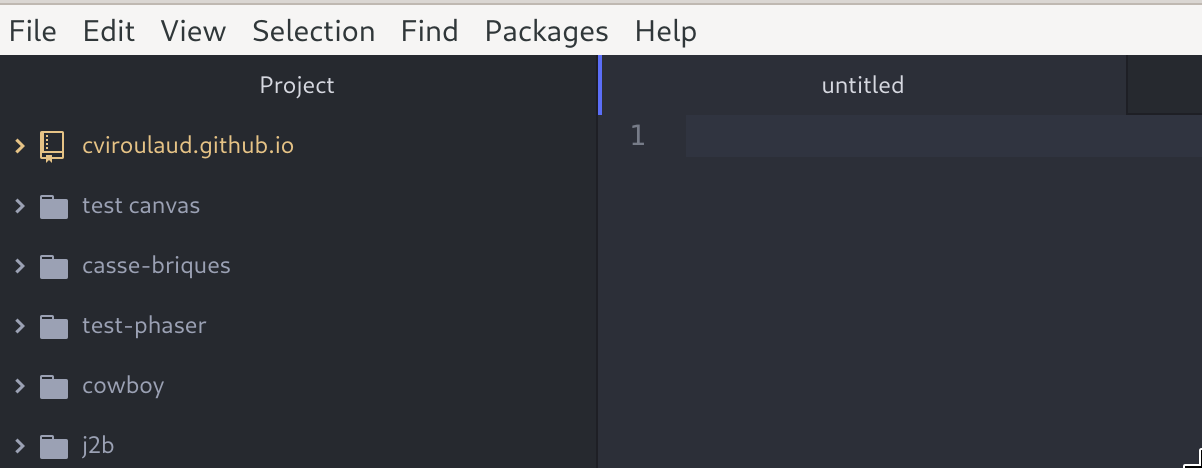
\includegraphics[width=8cm]{ressources/atom.png}
\captionof{figure}{Logiciel Atom}
\label{atom}
\end{center}
\item Si le panneau \emph{projects} n'est pas ouvert, sélectionner \emph{View/Toggle Tree View}.
\item Dans le panneau \emph{projects} faire un clic-droit puis choisir \emph{Add Project Folder}. Sélectionner le dossier crée précédemment.
\item Dans le panneau \emph{projects} faire un clic-droit sur le dossier puis sélectionner \emph{New File}.
\item Enregistrer ce fichier avec le nom \emph{index.html}
\end{enumerate}
\end{activite}

\section{Structure d'une page web}
\subsection{Langage de balises}
Le langage \emph{HTML} constitue les pages web. C'est un langage de balises c'est à dire que chaque composant de la page (texte, image, lien hypertexte...) est inséré grâce à des balises spécifiques. Les paragraphes suivants présentent certaines de ces balises.
\subsection{Le squelette}
Le code \ref{codemini} donne la structure minimale d'une page web.
\begin{code}[!h]
\begin{lstlisting}[language=html]
<html>
	<head>
	
	</head>
	<body>
	
	</body>
</html>
\end{lstlisting}
\captionof{code}{Page HTML minimale}
\label{codemini}
\end{code}

La plupart des blocs sont définis avec une \emph{balise ouvrante} (exemple: \emph{<html>)} et une \emph{balise fermante} (exemple: \emph{</html>}). On remarquera le bloc \emph{html} qui contient deux blocs:
\begin{itemize}
\item \textbf{head:} contiendra divers paramétrages pur la page. Il est possible de modifier le titre de la page.
\begin{lstlisting}[language=html]
<title>Mon titre</title>
\end{lstlisting}
\item \textbf{body:} contiendra les éléments qui s'afficheront sur la page. \textbf{Nous placerons tous nos futures balises dans ce bloc.}
\end{itemize}
\begin{activite}
\begin{enumerate}
\item Dans le fichier \emph{index.html}, commencer à écrire \emph{html}. Le sous-menu (figure \ref{html}) apparaît.
\item Appuyer sur la touche \emph{Entrée}. Le logiciel Atom crée automatiquement le squelette d'une page web. On remarquera quelques ajouts par rapport à la structure présentée dans le code \ref{codemini}.
\end{enumerate}
\end{activite}
\begin{figure}[!h]
\centering
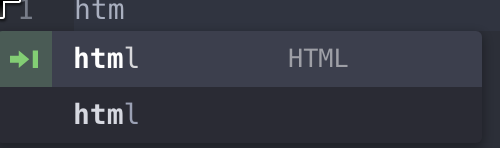
\includegraphics[width=5cm]{ressources/html.png}
\captionof{figure}{Auto-complétion}
\label{html}
\end{figure}


\subsection{Un paragraphe}
Chaque nouveau paragraphe sera inséré entre les balises \emph{<p>} et \emph{</p>}.
\begin{lstlisting}[language=html]
<p>Mon texte entre les balises.</p>
\end{lstlisting}
\subsection{Un titre}
Il existe six niveaux de titre: de \emph{h1} à \emph{h6}.
\begin{lstlisting}[language=html]
<h1>Un titre</h1>
<h2>Un sous-titre</h2>
\end{lstlisting}
\subsection{Une liste}
Elle permet d'énumérer plusieurs contenus. Il y a la balise \emph{ul} qui englobe la liste et \emph{li} pour chaque item.
\begin{lstlisting}[language=html]
<ul>
	<li>premier item</li>
	<li>deuxième item</li>
	<li>troisième item</li>
</ul>
\end{lstlisting}
\subsection{Un lien hypertexte}
C'est la base du web. Il est possible d'ouvrir une nouvelle page en cliquant sur un \emph{lien hypertexte}. Nous distinguerons deux:
\begin{itemize}
\item Ouvrir une page sur le même site. On utilisera un \emph{chemin relatif} c'est à dire qui part de la page actuelle vers la page à ouvrir.
\item Ouvrir un lien externe. On utilisera un \emph{chemin absolu} c'est à dire l'adresse complète de la nouvelle page.
\end{itemize}
\begin{lstlisting}[language=html]
<a href="autre-page.html">Lien vers une page du site</a>
<a href="https://lyceejaydebeaufort.fr/">Lien vers une page externe</a>
\end{lstlisting}
Nous remarquerons \emph{l'attribut href} à l'intérieur de la balise ouvrante \emph{a}.
\subsection{Une image}
Il n'y a pas de balise fermante pour une image. Il faut remarquer l'utilisation de l'attribut \emph{src} qui indique le chemin de l'image à afficher.
\begin{lstlisting}[language=html]
<img src="images/mon-image.jpg">
\end{lstlisting}
Dans ce cas, l'image \emph{mon-image.jpg} est stockée dans le répertoire \emph{images}. C'est une pratique que nous appliquerons également: afin d'ordonner les éléments nous rangerons les images dans un dossier \emph{images}.
\subsection{Pour aller plus loin}
Il existe de nombreuses balises pour construire une page web. La page \begin{center}
\url{https://developer.mozilla.org/fr/docs/Web/HTML/Element}
\end{center} recense de manière exhaustive les différentes balises.
\section{Création de la fiche de présentation}
Le logiciel \emph{Atom} permet de créer une page html. Une fois enregistrée, il faut ouvrir cette page avec un \emph{navigateur} comme Firefox. Il décode les instructions de la page html (code \ref{site}) et affiche le contenu (figure~\ref{rendu}).
\begin{activite}
Créer une page web du projet d'orientation. Cette page devra présenter:
\begin{itemize}
\item les spécialités envisagées pour l'année de première,
\item les études post-baccalauréat,
\item les idées de métier.
\end{itemize}
Il s'agit bien d'un projet. Les choix présentés sur cette page permettront d'établir une première réflexion sur l'avenir. Ainsi il faudra détailler les propositions données. Par exemple, un choix de métier pourra renvoyer vers une page ONISEP, une spécialité pourra être expliquée à travers un paragraphe ou une vidéo trouvée sur le web.
\\D'un point de vue technique elle devra contenir:
\begin{itemize}
\item un ou plusieurs titres,
\item un ou plusieurs paragraphes,
\item du contenu multimédia (image, vidéo...),
\item au moins deux hyperliens.
\end{itemize}
\end{activite}
\begin{code}[!h]
\begin{lstlisting}[language=html]
<!DOCTYPE html>
<html lang="fr" dir="ltr">
  <head>
    <meta charset="utf-8">
    <title>Ma fiche de présentation</title>
  </head>
  <body>
    <h1>Identité</h1>
    <p>Je suis Christophe Viroulaud, enseignant en NSI la meilleure discipline</p>
    <img src="images/nsi.png">
  </body>
</html>
\end{lstlisting}
\caption{Construction de la page}
\label{site}
\end{code}
\begin{figure}[!h]
\centering
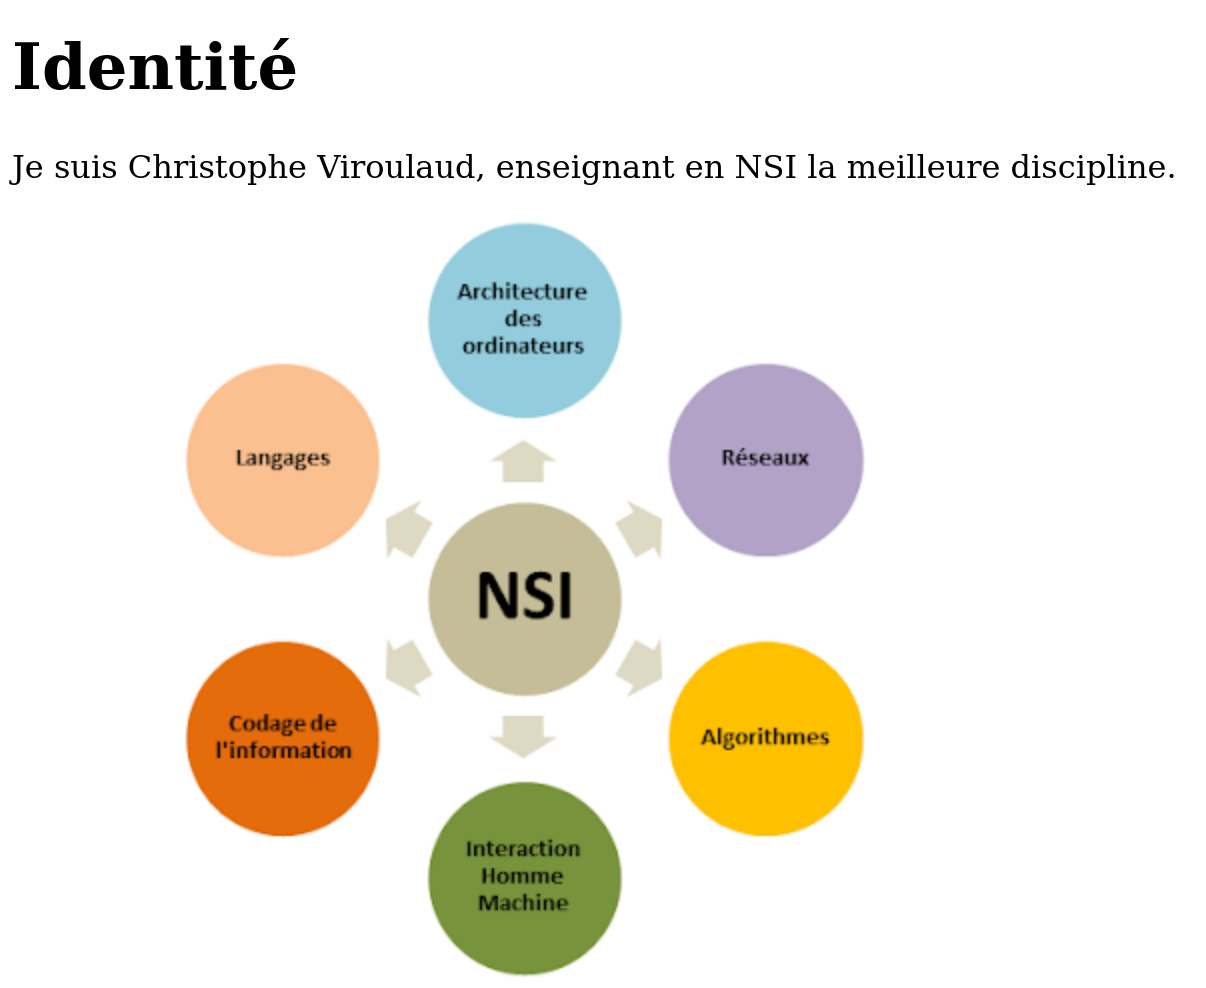
\includegraphics[width=10cm]{ressources/exemple-site.png}
\captionof{figure}{Rendu de la page sur Firefox}
\label{rendu}
\end{figure}
\end{Form}
\end{document}